\documentclass{article}
\usepackage[utf8]{inputenc}
\usepackage{amsmath}
\usepackage{amssymb}
\usepackage{xcolor}
\usepackage{tikz}
\usepackage{verbatim}
\usepackage{dirtytalk}
\usepackage{calc}

\usetikzlibrary{calc}

\title{CS4099}
\author{\vspace{-5ex}}
\date{\vspace{-5ex}}

\let\vec\mathbf
\newcommand{\norm}[1]{\left\lVert#1\right\rVert}

\begin{document}

\maketitle

\section{Week 2}

\paragraph{Control and output spaces}
The control space for robots is the wheels, and for neural nets the weights and biases.
The output space for robots is the movement/travel in the 2D obstacle space, and for neural nets the activation of the output layer.

\paragraph{The cost function}
Consider the output space
$$
    \vec{y} =
    \begin{bmatrix}
        y_{1} \\
        y_{2}
    \end{bmatrix}
    \in \mathbb{R}^2
.$$
The current weight configuration in the control space
$$
    \vec{w} =
    \begin{bmatrix}
        w_{1} \\
        w_{2} \\
        w_{3}
    \end{bmatrix}
    \in \mathbb{R}^3
$$
produces the initial output $\textcolor{blue}{i} \in \textbf{y}$. Our goal is $\textcolor{red}{g}  \in \textbf{y}$.




\begin{figure}[h]

    \begin{tikzpicture}

        \draw[thick, <->]
            (0, 5.5) node(y2line)[above] {$y_2$}
            |- (10, 0) node(y1line)[right] {$y_1$};

        \coordinate (i) at (2, 3);
        \coordinate (g) at (9, 3);
        \coordinate (frac_progress) at ($(i)!2cm!(g)$);
        \coordinate (frac_line_a) at (frac_progress |- y2line);
        \coordinate (frac_line_b) at (frac_progress |- y1line);

        \coordinate (dw_1) at ($(i)+(45:2cm)$);
        \coordinate (dw_2) at ($(i)+(-20:2cm)$);
        \coordinate (dw_3) at ($(i)+(-60:-2cm)$);
        \coordinate (dw_3_actual) at ($(i)+(-60:2cm)$);

        \draw[->] (i) -- (dw_1) node[above left] {$\frac{\delta \vec{y}}{\delta w_1}$};
        \draw[->] (i) -- (dw_2) node[below] {$\frac{\delta \vec{y}}{\delta w_2}$};
        \draw[->] (i) -- (dw_3) node[above] {$\frac{\delta \vec{y}}{\delta w_3}$};
        \draw[->, cyan] (i) -- (frac_progress);

        \draw[dotted, cyan] (frac_line_a) -- (frac_line_b);
        \draw[dotted] (dw_1 |- y2line) -- (dw_1 |- y1line);
        \draw[dotted] (dw_2 |- y2line) -- (dw_2 |- y1line);
        \draw[dotted] (dw_3_actual |- y2line) -- (dw_3_actual |- y1line);

        \draw[dashed] (i) -- (dw_1) -- (g);
        \draw[dashed] (i) -- (dw_2) -- (g);
        \draw[dashed] (i) -- (dw_3_actual) -- (g);
        \draw[->, dashed, cyan] (i) -- (g);

        \fill[blue] (i) circle (2pt) node[left] {$i$};
        \fill[red] (g) circle (2pt) node[right] {$g$};

    \end{tikzpicture}

    \caption{Diagram of the output space.}

\end{figure}



We define the cost function as
\begin{equation}
    C\left( \vec{w} \right) = \frac{\text{fractional progress}}{\text{total Euclidean distance}}.
\end{equation}

The \textcolor{cyan}{straight line goal-connecting path} would minimize the Euclidean distance while maximizing the fractional progress.




\section{Week 3}

\subsection{Research}
\paragraph{Simulated annealing}
This refers to a process that will temporarily accept sub-optimal (worse) values in hopes of overcoming local maxima, to reach better local minima.

\paragraph{Adam optimizer}
The name means \say{ADAptive Moment estimation}.
Instead of using a global learning rate (as in SGD), Adam \say{computes individual adaptive learning rates for different parameters from estimates of first and second moments of the gradients} \cite{adam}, i.e. the mean and variance.

\paragraph{The stripe problem in literature}
To do

\subsection{Experimentation}

\subsubsection{A problem that always achieves a point on the goal line (gradient of weights are at right angle)}

Consider the neural network below. Note that it does not have an activation function.

\begin{figure}[h]
    \begin{center}
        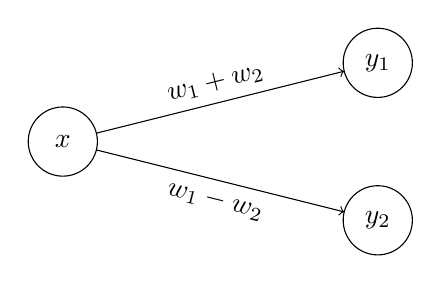
\begin{tikzpicture}
            [
                neuron/.style = {draw, circle, minimum size=25pt, inner sep=0pt, outer sep=0pt},
            ]
            
            \node [neuron] (x)  at (0,0) {$x$};
            \node [neuron] (y1) at (4,1) {$y_1$};
            \node [neuron] (y2) at (4,-1) {$y_2$};
            \draw[->] (x) -- (y1) node[midway, above, sloped] {$w_1 + w_2$};
            \draw[->] (x) -- (y2) node[midway, below, sloped] {$w_1 - w_2$};
        \end{tikzpicture}
    \end{center}
    \caption{The neural network.}
\end{figure}

Here we have
\begin{equation*}
    \vec{y}(x; \vec{w}) = 
    \begin{bmatrix}
        w_1 + w_2 \\
        w_1 - w_2
    \end{bmatrix}
    x
\end{equation*}
with the derivative
\begin{equation*}
    \frac{\partial \vec{y}}{\partial \vec{w}}
    =
    \begin{bmatrix}
        \frac{\partial y_1}{\partial w_1} & \frac{\partial y_1}{\partial w_2} \\
        \frac{\partial y_2}{\partial w_1} & \frac{\partial y_2}{\partial w_2}
    \end{bmatrix}
    =
    \begin{bmatrix}
        1 & 1 \\
        1 & -1
    \end{bmatrix}
    x.
\end{equation*}

For
$x = 1$,
let our goal be $\vec{g} = \begin{bmatrix} 10 \\ 2 \end{bmatrix}$
and the initial weight configuration be
$\vec{w} = \begin{bmatrix} 3 \\ 1 \end{bmatrix}$.
This leads to the current position $\vec{p} = \begin{bmatrix} 4 \\ 2 \end{bmatrix}$ in output space.

Say we want to achieve $\frac{1}{6}$ fractional progress, so we aim to achieve the point $\vec{q}$ at the intersection of the fractional progress line with the goal line in the diagram below. 


\begin{figure}[h]
    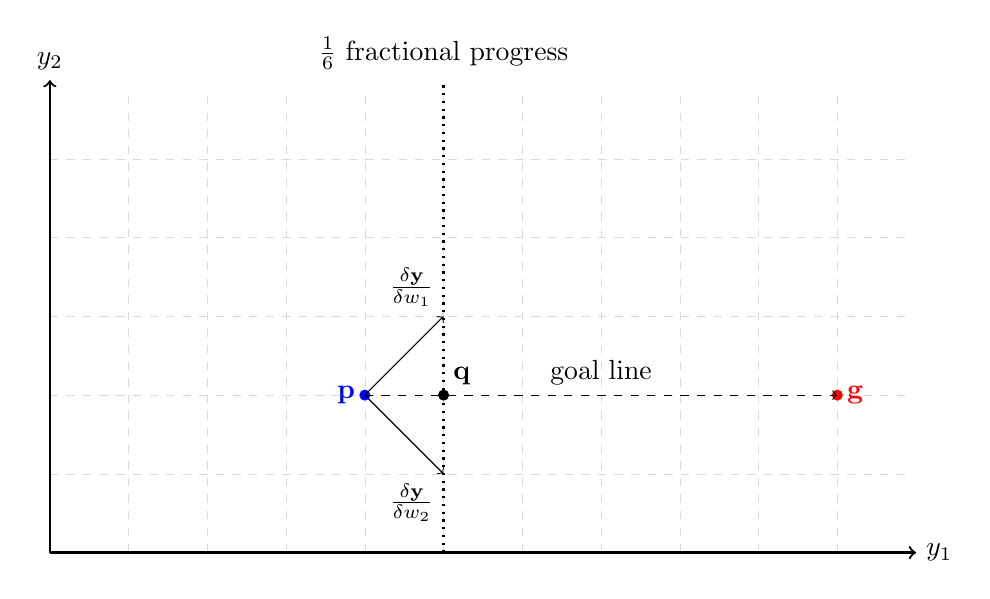
\begin{tikzpicture}
        
        \draw[help lines, color=gray!30, dashed] (0, 5.9) grid (10.9, 0);
        \draw[thick, ->] (0, 0) -- (11, 0) node[right] {$y_1$};
        \draw[thick, ->] (0, 0) -- (0, 6) node[above] {$y_2$};
        
        \coordinate (p) at (4, 2);
        \coordinate (g) at (10, 2);
        \coordinate (dw_1) at (1, 1);
        \coordinate (dw_2) at (1, -1);
        \coordinate (q) at (5, 2);
        
        \fill[blue] (p) circle (2pt) node[left] {$\vec{p}$};
        \fill[red] (g) circle (2pt) node[right] {$\vec{g}$};
        \fill (q) circle (2pt) node[above right] {$\vec{q}$};
        
        \draw[->] (p) -- +(dw_1) node[above left] {$\frac{\delta \vec{y}}{\delta w_1}$};
        \draw[->] (p) -- +(dw_2) node[below left] {$\frac{\delta \vec{y}}{\delta w_2}$};
        \draw[thick, dotted] (5, 0) -- (5, 6) node[above] {$\frac{1}{6}$ fractional progress};
        \draw[->, dashed] (p) -- (g) node[midway, above] {goal line};

    \end{tikzpicture}

    \caption{Diagram of the weights' partial derivatives in output space along with the sub-goal.}
\end{figure}

Now we need to find out by how much we need to update $\vec{w}$. In other words, we need to find $\vec{a} \in \mathbb{R}^2$ so that after
\begin{equation}
    \label{update_w}
    \vec{w} \leftarrow \vec{w} + \vec{a}
\end{equation}
we get
\begin{equation*}
    \vec{y}(1; \vec{w}) =
    \begin{bmatrix}
        4 \\
        2
    \end{bmatrix} + 
    \begin{bmatrix}
        1 \\
        0
    \end{bmatrix}.
\end{equation*}

This is equivalent to finding the vector $\vec{a} = \begin{bmatrix} a_1 \\ a_2 \end{bmatrix}$ that satisfies
\begin{align*}
    \begin{bmatrix}
        1 \\
        0
    \end{bmatrix}
    &=
    \frac{\partial \vec{y}}{\partial \vec{w}} \cdot \vec{a}
    \\
    &=
    a_1
    \frac{\partial \vec{y}}{\partial w_1}
    +
    a_2
    \frac{\partial \vec{y}}{\partial w_2}
    \\
    &=
    a_1
    \begin{bmatrix}
        1 \\
        1
    \end{bmatrix}
    +
    a_2
    \begin{bmatrix}
        1 \\
        -1
    \end{bmatrix},
\end{align*}
so
\begin{align*}
    a_1 = a_2 = \frac{1}{2} \\
    \vec{a} =
    \frac{1}{2}
    \begin{bmatrix}
        1 \\
        1
    \end{bmatrix}.
\end{align*}

Using (\ref{update_w}), we update $\vec{w}$ to
\begin{equation*}
    \vec{w}
    \leftarrow
    \begin{bmatrix}
        3 \\
        1
    \end{bmatrix}
    +
    \frac{1}{2}
    \begin{bmatrix}
        1 \\
        1
    \end{bmatrix}
    =
    \frac{1}{2}
    \begin{bmatrix}
        7 \\
        3
    \end{bmatrix}.
\end{equation*}


Now let's see what we get for the new $\vec{q}$ in this updated system:
\begin{equation*}
    \vec{q} =
    \vec{y}(1; \vec{w}) =
    \begin{bmatrix}
        w_1 + w_2 \\
        w_1 - w_2
    \end{bmatrix} = 
    \frac{1}{2}
    \begin{bmatrix}
        7+3 \\
        7-3
    \end{bmatrix}
    =
    \begin{bmatrix}
        5 \\
        2
    \end{bmatrix}
\end{equation*}
which is correct (see diagram).

\paragraph{Remarks:}
In this very simple example, we can use linear algebra to deterministically reach our sub-goal. 
However, as soon as we have three weights, there will be more than one possible vector $\vec{a} \in \mathbb{R}^3$ that achieves the sub-goal. 
Are there any drawbacks for choosing a particular $\vec{a}$ over another, if there are multiple options?

Furthermore, this network is so simple that the partial derivatives of the weights with respect to the output space aren't dependent on the weights themselves. However, in a \say{real} neural network, the gradients will influence each other because they depend on the weights. What happens in that case? (This question is examined in the next section.)

\subsubsection{When gradients are dependent on other weights}
Consider the neural network below. It uses the ReLU activation function.

\begin{figure}[h]
    \begin{center}
        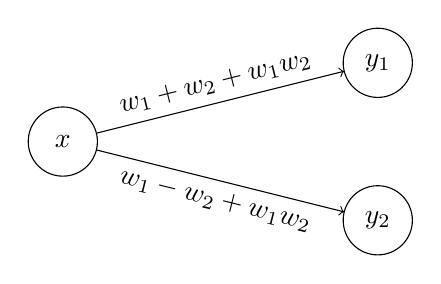
\begin{tikzpicture}
            [
                neuron/.style = {draw, circle, minimum size=25pt, inner sep=0pt, outer sep=0pt},
            ]
            
            \node [neuron] (x)  at (0,0) {$x$};
            \node [neuron] (y1) at (4,1) {$y_1$};
            \node [neuron] (y2) at (4,-1) {$y_2$};
            \draw[->] (x) -- (y1) node[midway, above, sloped] {$w_1 + w_2 + w_1 w_2$};
            \draw[->] (x) -- (y2) node[midway, below, sloped] {$w_1 - w_2 + w_1 w_2$};
        \end{tikzpicture}
    \end{center}
    \caption{The neural network.}
\end{figure}

Here we have
\begin{equation*}
    \vec{y}(x; \vec{w}) = 
    \begin{bmatrix}
        \max \left( 0, w_1 + w_2 + w_1 w_2 \right) \\
        \max \left( 0, w_1 - w_2 + w_1 w_2 \right)
    \end{bmatrix}
    x
\end{equation*}
with the derivative
\begin{equation*}
    \frac{\partial \vec{y}}{\partial \vec{w}}
    =
    \begin{bmatrix}
        \max(0, w_2 + 1) & \max(0, w_1 + 1) \\
        \max(0, w_2 + 1) & \max(0, w_1 - 1)
    \end{bmatrix}
    x.
\end{equation*}

For
$x = 1$,
let our goal be $\vec{g} = \begin{bmatrix} 9 \\ 1 \end{bmatrix}$
and the initial weight configuration be
$\vec{w} = \begin{bmatrix} 1 \\ 1 \end{bmatrix}$.
This leads to the current position $\vec{p} = \begin{bmatrix} 3 \\ 1 \end{bmatrix}$ in output space.


\begin{figure}[h]
    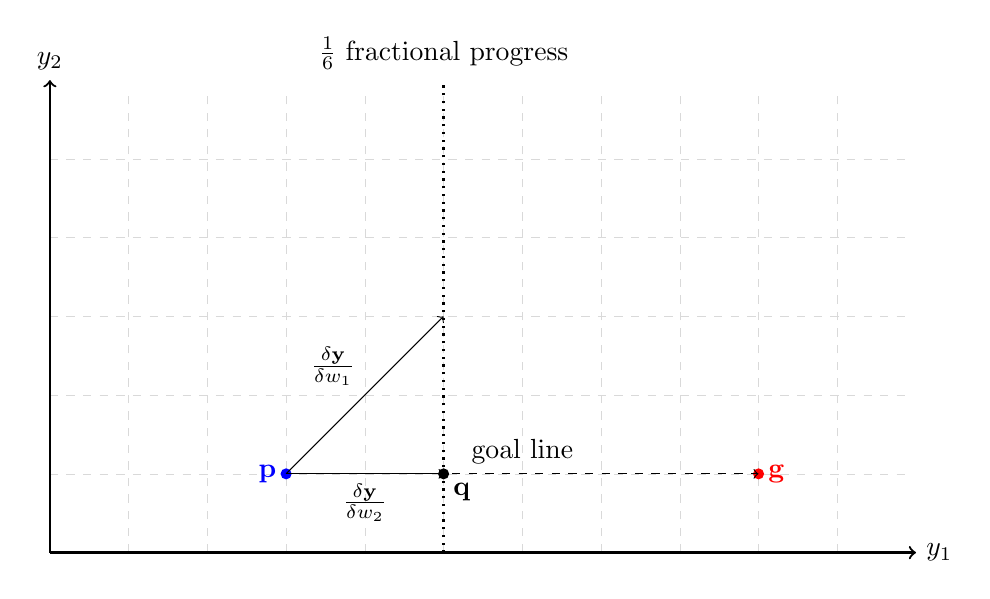
\begin{tikzpicture}
        
        \draw[help lines, color=gray!30, dashed] (0, 5.9) grid (10.9, 0);
        \draw[thick, ->] (0, 0) -- (11, 0) node[right] {$y_1$};
        \draw[thick, ->] (0, 0) -- (0, 6) node[above] {$y_2$};
        
        \coordinate (p) at (3, 1);
        \coordinate (g) at (9, 1);
        \coordinate (dw_1) at (2, 2);
        \coordinate (dw_2) at (2, 0);
        \coordinate (q) at (5, 1);
        
        \fill[blue] (p) circle (2pt) node[left] {$\vec{p}$};
        \fill[red] (g) circle (2pt) node[right] {$\vec{g}$};
        \fill (q) circle (2pt) node[below right] {$\vec{q}$};
        
        \draw[->] (p) -- +(dw_1) node[midway, above left] {$\frac{\delta \vec{y}}{\delta w_1}$};
        \draw[->] (p) -- +(dw_2) node[midway, below] {$\frac{\delta \vec{y}}{\delta w_2}$};
        \draw[thick, dotted] (5, 0) -- (5, 6) node[above] {$\frac{1}{6}$ fractional progress};
        \draw[->, dashed] (p) -- (g) node[midway, above] {goal line};

    \end{tikzpicture}

    \caption{Diagram of the weights' partial derivatives in output space along with the sub-goal.}
\end{figure}

Just looking at the diagram, one could guess to update the weights as follows to achieve $\vec{q}$:
\begin{equation*}
    \vec{w} \leftarrow \vec{w} +
    \begin{bmatrix}
        0 \\
        1
    \end{bmatrix}.
\end{equation*}
Using $\Vec{w} = \begin{bmatrix} 1 \\ 2 \end{bmatrix}$, we calculate the new output
\begin{equation*}
    \vec{y}(1; \vec{w})
    = 
    \begin{bmatrix}
        \max \left( 0, 1 + 2 + 2 \right) \\
        \max \left( 0, 1 - 2 + 2 \right)
    \end{bmatrix}
    =
    \begin{bmatrix}
        5 \\
        3
    \end{bmatrix}
\end{equation*}
which is \textit{not} our sub-goal $\vec{p}$! The reason for this is that unlike the previous network, the partial derivative $\frac{\partial \vec{y}}{\partial w_1}$ is dependent on the value of $w_2$ and vice-versa.

\paragraph{Remarks:}
When the partial derivatives are functions of each other (i.e. depend on each other), we can't use simple linear algebra in order to find the combination of the weights to achieve a specific subgoal. 
This makes intuitive sense, because if it were possible, we could simply choose the goal as our subgoal and expect to use linear algebra to find the optimum weight configuration which would eliminate the need for training neural networks.

\subsubsection{A problem with an unrealizable goal line, but realizable goal}
Did not find a good example yet.


\section{Week 5}

\subsection{Research}

\paragraph{Radial basis function}
A radial basis function is a real-valued function $f$ that satisfies the property $f(\vec{x}) = f(\norm{\vec{x}})$. 
RBFs are used as a kernel in SVMs. 
They are infinitely differentiable.

Two commonly used RBFs are the Gaussian function
$$ f(x) = e^{-x^2} $$
and the bump function
$$ f(x) = 
\begin{cases}
    e^{-\frac{1}{1-x^2}} & \text{for $-1<x<1$} \\
    0 & \text{otherwise}.
\end{cases}
$$

\subsection{Experimentation}

\subsubsection{Replicating the simple neural network with the shallow excitation gradient}
Consider the very simple neural network below. 
\begin{figure}[h]
    \begin{center}
        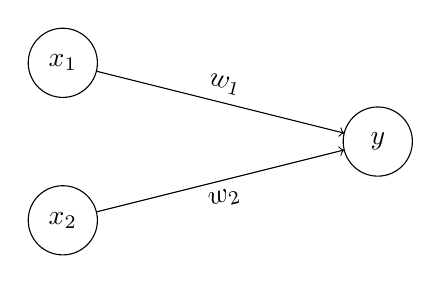
\begin{tikzpicture}
            [
                neuron/.style = {draw, circle, minimum size=25pt, inner sep=0pt, outer sep=0pt},
            ]
            
            \node [neuron] (x1)  at (0,2) {$x_1$};
            \node [neuron] (x2) at (0,0) {$x_2$};
            \node [neuron] (y) at (4,1) {$y$};
            \draw[->] (x1) -- (y) node[midway, above, sloped] {$w_1$};
            \draw[->] (x2) -- (y) node[midway, below, sloped] {$w_2$};
        \end{tikzpicture}
    \end{center}
    \caption{The neural network.}
\end{figure}

The output neuron's excitation is given by 
\begin{equation*}
    y(\vec{x}; \vec{w}, b) = \vec{w} \vec{x} + b.
\end{equation*}

Consider the two points in input space
$\vec{a} = 
\begin{bmatrix}
    0.6 \\ 0.4
\end{bmatrix}$
and
$\vec{b} = 
\begin{bmatrix}
    1 \\ 0.4
\end{bmatrix}$
with the targets $y(\vec{a}) = 0.2$ and $y(\vec{b}) = 0.8$.

The current weight configuration should be such that the hyperplane in output space of the 0.5 excitation line should be given by $x_1=0.5$.
Furthermore, the current activations should be $y(\vec{a}) = 0.51$ and $y(\vec{b}) = 0.55$ such that we get the configuration outlined in Fig. \ref{week5:initial}.
\begin{figure}[h]

    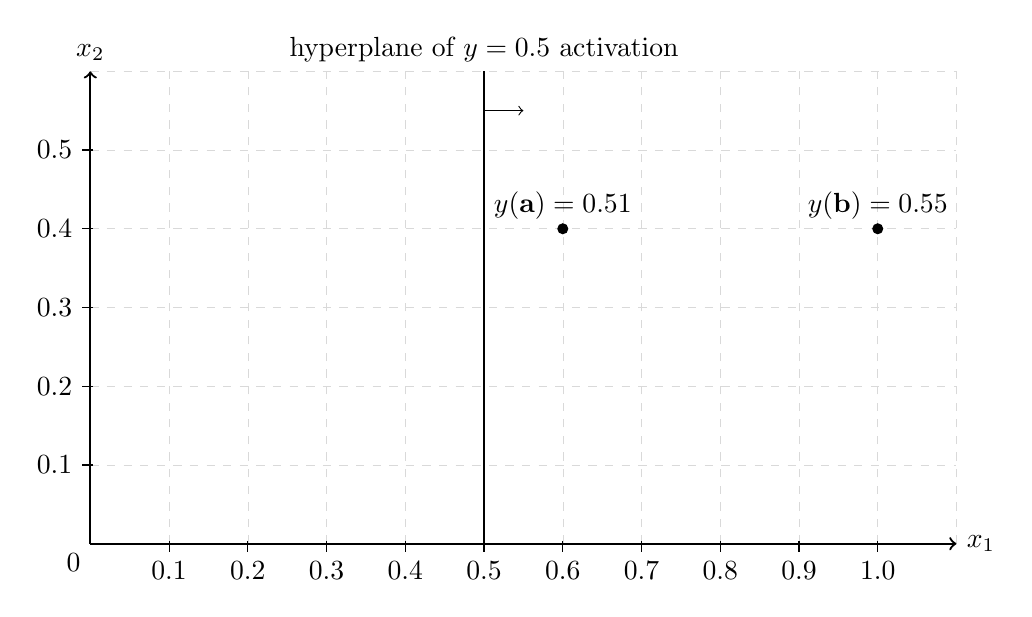
\begin{tikzpicture}[x=10cm,y=10cm]
        
        \draw[help lines, color=gray!30, dashed] (0, .6) grid (1.1, 0);
        \draw[thick, ->] (0, 0) -- (1.1, 0) node[right] {$x_1$};
        \draw[thick, ->] (0, 0) -- (0, .6) node[above] {$x_2$};
        \foreach \x in {0.1, 0.2, 0.3, 0.4, 0.5, 0.6, 0.7, 0.8, 0.9, 1.0 }
     		\draw (\x,1pt) -- (\x,-3pt)
            node[anchor=north] {\x};
        \foreach \y in {0.1, 0.2, 0.3, 0.4, 0.5 }
            \draw (1pt,\y) -- (-3pt,\y)
           node[anchor=east] {\y};
        \draw (0, 0) node[below left] {0};
        
        \draw (0.5, 0) -- (.5, .6) node[above] {hyperplane of $y=0.5$ activation};
        
        \coordinate (a) at (.6, .4);
        \coordinate (b) at (1, .4);
        
        \fill (a) circle (2pt) node[above] {$y(\vec{a})=0.51$};
        \fill (b) circle (2pt) node[above] {$y(\vec{b})=0.55$};

        \draw[->] (.5, .55) -- (.55, .55);
    \end{tikzpicture}

    \caption{The initial configuration with the hyperplane. The arrow is pointing in the direction of increasing activation.}
    \label{week5:initial}
\end{figure}

After some experimentation, it was established that this configuration can be achieved using
$\vec{w} = \begin{bmatrix}
    0.1 \\ 0.0005
\end{bmatrix}$
and $b = 0.45$ thus leading to the function
\begin{equation*}
    y(\vec{x}) = 0.1 x_1 + 0.0005 x_2 + 0.45.
\end{equation*}

\paragraph{Remarks:}
To get a gradient this shallow, it was necessary to introduce a third parameter $b$. 
We need to investigate whether we can call it a \say{non-trainable variable}, so we effectively only have two weights.

\bibliographystyle{apalike}
\bibliography{bibliography}

\end{document}